%%%%%%%%%%%%%%%%%%%%%%%%%%%%%%%%%%%%%%%%%%%%%%%%%%%%%%%%%%%%%%%%%%%%%%%%%%%%%%%%%
%% Fridolin Pokorny (fridex)
%%%%%%%%%%%%%%%%%%%%%%%%%%%%%%%%%%%%%%%%%%%%%%%%%%%%%%%%%%%%%%%%%%%%%%%%%%%%%%%%%
\documentclass[compress]{beamer}
\usepackage[english]{babel}
\usepackage[utf8]{inputenc}
\usepackage{graphics}
\usepackage{hyperref}

\usetheme{Boadilla}

\begin{document}

\title{Rozpoznání žil prstu}
%\subtitle{using BEAMER class for \LaTeX}
\author{Tomáš Rajca \& Fridolín Pokorný}
%\institute{}
%\titlegraphic{}
\date{\today}

%%%%%%%%%%%%%%%%%%%%%%%%%%%%%%%%%%%%%%%%%%%%%%%%%%%%%%%%%%%%%%%%%%%%%%%%%%%%%%%%

\begin{frame}[plain]
  \titlepage
\end{frame}

%%%%%%%%%%%%%%%%%%%%%%%%%%%%%%%%%%%%%%%%%%%%%%%%%%%%%%%%%%%%%%%%%%%%%%%%%%%%%%%%
%%%%%%%%%%%%%%%%%%%%%%%%%%%%%%%%%%%%%%%%%%%%%%%%%%%%%%%%%%%%%%%%%%%%%%%%%%%%%%%%
%%%%%%%%%%%%%%%%%%%%%%%%%%%%%%%%%%%%%%%%%%%%%%%%%%%%%%%%%%%%%%%%%%%%%%%%%%%%%%%%

\begin{frame}
  \frametitle{Realizácia}
  \begin{itemize}
    \item rozpoznať na základe snímkov (128 snímkov, 7 ľudí x 18 snímkov)
    \item implementovaných 5 algoritmov\,--\,postupné zdokonaľovanie
    \item porovnanie s existujúcimi nástrojmi
  \end{itemize}
\begin{figure}[ht!]
	\centering
	
\includegraphics[width=1.5cm]{../fig/A_18.eps}
	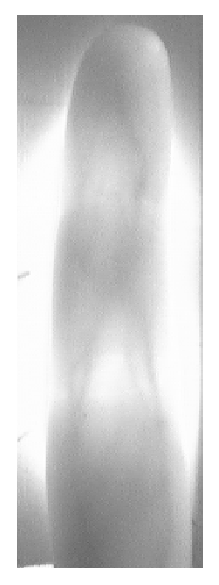
\includegraphics[width=1.5cm]{../fig/A_10.eps}
	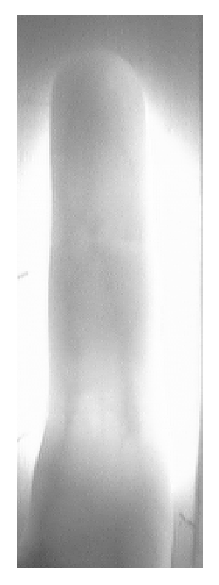
\includegraphics[width=1.5cm]{../fig/A_12.eps}
\end{figure}
\end{frame}

\begin{frame}
  \frametitle{Algoritmy}
  \begin{itemize}
    \item \emph{Alg1}\,--\,prosté porovnanie hodnôt pixelov
    \item \emph{Alg2}\,--\,úprava histogramu
    \item \emph{Alg3}\,--\,detekcia obrysov prstu
    \item \emph{Alg4}\,--\,počet priesečníkov úsečky (úsečka \texttt{x} žila)
    \item \emph{Alg5}\,--\,fused
  \end{itemize}
\end{frame}

\begin{frame}
\frametitle{Výsledky}
\begin{figure}[ht!]
	\centering
	
\includegraphics[width=8cm]{../fig/all.eps}
	\caption{\label{fig:all} DET a ROC krivky všetkých implementovaných algoritmov}
\end{figure}
\end{frame}

\begin{frame}
\begin{figure}[ht!]
	\centering
	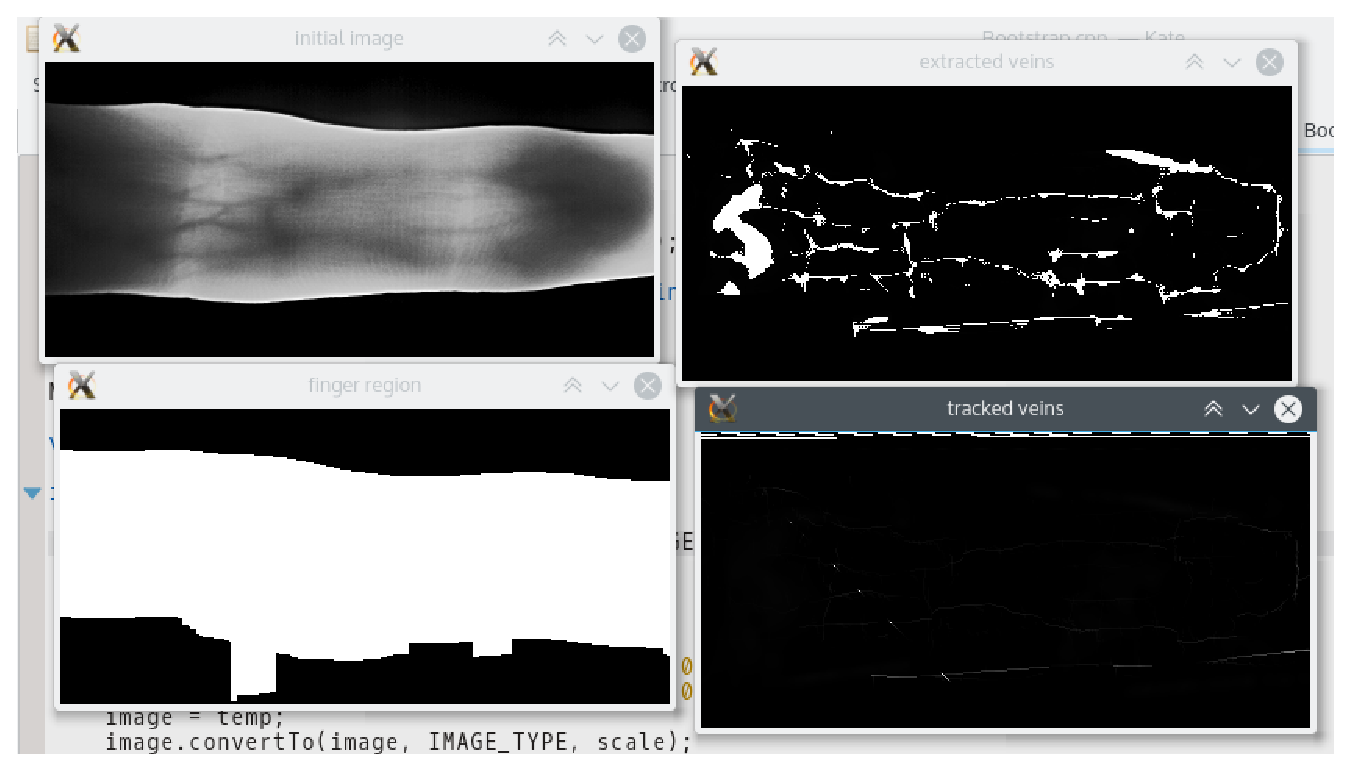
\includegraphics[width=12cm]{../fig/test_orig.eps}
\end{figure}
\end{frame}

\begin{frame}
\begin{figure}[ht!]
	\centering
	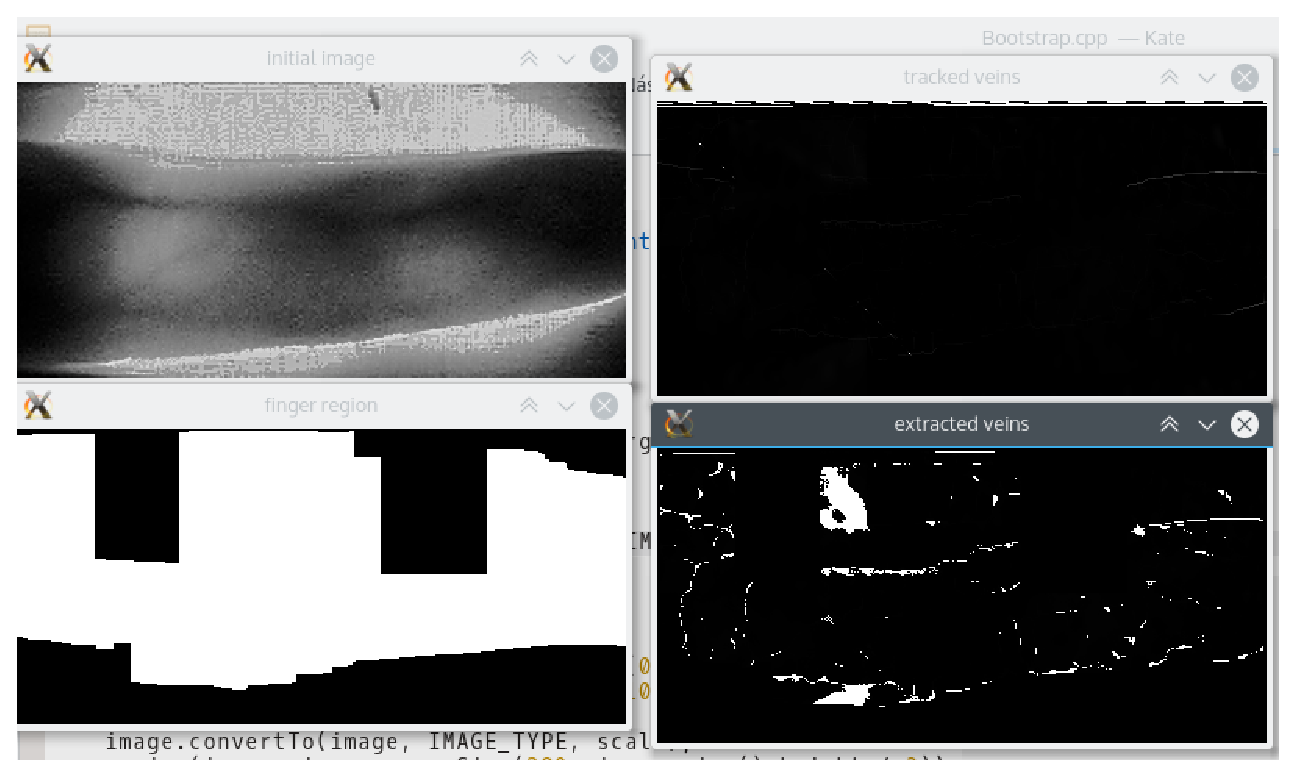
\includegraphics[width=12cm]{../fig/test_nas.eps}
\end{figure}
\end{frame}


%%%%%%%%%%%%%%%%%%%%%%%%%%%%%%%%%%%%%%%%%%%%%%%%%%%%%%%%%%%%%%%%%%%%%%%%%%%%%%%%
%%%%%%%%%%%%%%%%%%%%%%%%%%%%%%%%%%%%%%%%%%%%%%%%%%%%%%%%%%%%%%%%%%%%%%%%%%%%%%%%

\part{bib}
\subsection{Bibliography}
\begin{frame}
\begin{thebibliography}{10}
\bibitem{konalio}
	Kupidura P.,
	\emph{System for human identification based on finger vein pattern},
	[online: \url{https://github.com/konalio/FingerVeinRecognition}],
	[cite: 6.12.2015].
\bibitem{mahri}
	Nurhafizah M., Sundi S. A., Bakhtiar A. R.,
		\emph{Finger Vein Recognition Algorithm Using Phase Only Correlation},
	[online: \url{http://citeseerx.ist.psu.edu/viewdoc/download?doi=10.1.1.476.8969&rep=rep1&type=pdf}],
	[cite: 6.12.2015].

\end{thebibliography}
\end{frame}

\end{document}

